\chapter{Онолын судалгаа}
Онолын судалгаа бүлгийн хүрээнд блокчэйн технологи болон дижитал эрхийн менежментийн талаар судлах мөн цахим бүтээлийн лицензийн төвлөрсөн бус системтэй ижил төстэй системүүд болон, энэхүү сэдвээр судалгааны ажил хийгдсэн эсэхийг судалж хооронд нь харьцуулалт хийх бөгөөд үүний үр дүнд системийн хэрэгцээ шаардлага, давуу тал, өөр ямар нэмэлт боломжууд байж болох талаар мэдэх юм. Мөн системийг хөгжүүлэхэд шаардагдах технологи болон фреймворкуудын талаарх судалгааг хийлээ.

\section{Блокчэйн технологи}
Хамгийн анх блокчэйн технологийн талаар 2008 онд Сатоши Накамото
гэдэг этгээдийн нийтэлсэн “Биткойн: Peer-to-Peer Электрон Мөнгөний Тогтолцоо” судалгааны ажлын нийтлэлд дурдагдсан байдаг \cite{blockchain}.

Блокчэйн гэдэг нь өгөгдөл буюу дата мэдээллүүдийг хадгалдаг нэгэн төрлийн мэдээллийн бааз гэж хэлж болно. Бааз доторх дата мэдээллийг Блок гэж нэрлэгдэх хэсгүүдэд багцлан хадгалж уг сүлжээнд холбогдсон бүх компьютерт ижил хуулбар болгон тархмал хэлбэрээр хадгална. Тэдгээр блокуудыг өөр хоорондоо гинжин хэлхээ буюу математик тооцоолол, цахим нууцлалын аргаар хэлхэн холбосноор бидний ярьж буй Блокчэйн үүсэх юм.

\subsection{Блокчэйний онцлог}
\textbf{Тархсан Peer-to-Peer (P2P)} сүлжээ гэдэг нь сүлжээнд оролцогч буюу зангилаанууд нь газарзүйн хувьд тархсан байдаг ба аль ч хоёр зангилаа хоорондоо байршлаас үл хамааран ямар нэг серверээр дамжилгүйгээр өөр хоорондоо шууд холбогддог сүлжээ юм.

\textbf{Tархсан бүртгэлийн дэвтэр буюу Distributed ledger technology (DLT)} технологи нь мэдээллийг тархсан P2P сүлжээний оролцогч нар дээр хадгалдаг технологи бөгөөд уламжлалт өгөгдлийн сангийн системээс ялгарах гол ялгаа нь төвлөрсөн өгөгдлийн сан болон төвлөрсөн удирдлагын функц байхгүйд оршино \cite{dlt}.

Блокчэйн нь DLT технологийн гол төлөөлөгч бөгөөд мэдээллийн гинжин хэлхээ юм. Блокчэйнд тогтсон хэмжээтэй блок үүсгэж, үүн дотроо мэдээллийг хадгалах ба эхний блок дүүрэхэд дараагийн шинэ блок үүсгэдэг. Эдгээр блок нь хэш функцээр кодлогдсон байх ба блокийг цаг хугацааны дагуу жагсааж, блок тус бүр яг өөрийн өмнөх блокийн мэдээллийг өөр дотроо хадгалах байдлаар гинжин бүтцийг үүсгэнэ.

Блокчэйн технологийн хамгийн чухал, онцлох давуу тал нь төвлөрсөн бус тархсан бүтэцтэй бөгөөд сүлжээнд байгаа бүх компьютер блокчэйний халдашгүй чанарыг үргэлж баталгаажуулж байдаг ба хэн нэгэн, эсвэл аль нэг компани үүн доторх өгөгдөл түүний бүрэн бүтэн байдлыг удирдах боломжгүй байдагт байгаа юм. Блокчэйний бүх зангилаа ижил мэдээллийг агуулж байдаг болохоор “A” зангилаан дахь өгөгдөл эвдэрч гэмтвэл блокчэйний хэсэг болж чадахгүй, учир нь өгөгдөл нь бусад “B” болон “C” зангилааны өгөгдөлтэй ижил байж чадахгүй болно.

\begin{figure}[h]
	\centering
	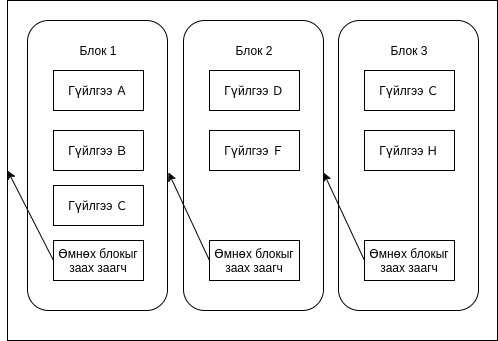
\includegraphics[scale=0.6]{src/images/blockchain-structure.jpg}
	\caption{Блокчэйний өгөгдлийн бүтэц}
\end{figure}

\subsection{Блокчэйний нууцлалын технологи}
\subsubsection{Криптограф хэш}
Криптограф хэш функц нь оруулсан өгөгдлийн уртаас үл хамааран тогтсон урттай хэш утгуудыг буцаадаг. Оролтын зөвхөн нэг тэмдэгт өөрчлөгдөхөд гаралтын хэш утгууд нь эрс ялгаатай байна. Энэ шинж чанарыг ашиглан, гүйлгээний өгөгдөл болон бусад бүх өгөгдлийн хувьд засвар ороогүй болохыг баталгаажуулах боломжийг олгодог.
Жишээ нь, та Mac-ын командлайнаар дараах командыг оруулбал, SHA-256 hash функцийн утгыг хялбархан олох болно.

\begin{figure}[h]
	\centering
	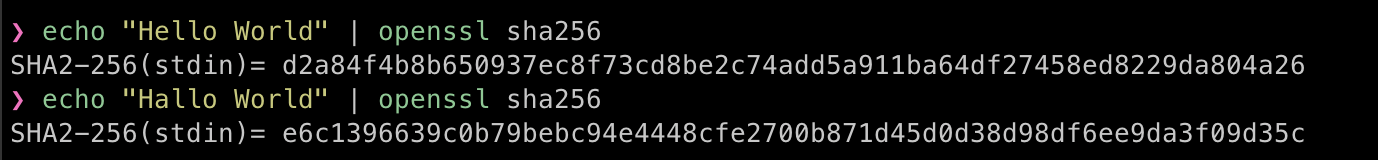
\includegraphics[scale=0.36]{src/images/hash-example.png}
	\caption{"Hello World", "Hallo World" гэсэн үгнүүдийн хэшийг бодсон байдал}
\end{figure}

"Hello World", "Hallo World" гэсэн үгнүүдийн sha256 хэшийг бодсон байдал жишээн дээр, "Hello World" гэсэн үгний SHA-256 hash утга болон, "e"-г "a"-гээр сольсон үгийн SHA-256 hash утгыг харуулсан байна. Зөвхөн нэг үсгээр ялгаатай боловч, тэдгээрийн hash утгууд нь эрс ялгаатай байна. Энэ мэтчилэн hash функц нь оролт нь 1 байтаар л ялгаатай байхад, эрс өөр үр дүн гаргадаг шинж чанарыг агуулж байдаг. Энэ шинж чанарыг ашиглан, гүйлгээний өгөгдөл болон тэдгээрийг хадгалах блокийн бүх өгөгдлийн хувьд гарах hash утгыг тухайн өгөгдлийн бүтцэд оруулснаар, засвар ороогүй болохыг баталгаажуулах боломжтой болно.

\subsubsection{Тоон гарын үсэг}
Тоон гарын үсэг нь дижитал мессеж эсвэл баримт бичгийн жинхэнэ эсэхийг шалгах математик аргачлал юм. Энэ нь хос түлхүүр үүсгэх замаар ажилладаг: өргөн тархсан нийтийн түлхүүр, нууцлагдсан хувийн түлхүүр. Гарын үсэг зурахдаа баримт бичгийн өвөрмөц хэшийг үүсгэж, хувийн түлхүүрээр шифрлэж, тоон гарын үсгийг бүрдүүлдэг. Хүлээн авсны дараа хэшийг илгээгчийн нийтийн түлхүүрээр тайлж, хүлээн авсан баримтаас шинэ хэш үүсгэнэ. Хэрэв хоёулаа таарч байвал энэ нь тухайн баримт бичиг нь жинхэнэ бөгөөд ямар нэгэн өөрчлөлт ороогүй гэсэн үг юм.

\begin{figure}[h!]
	\centering
	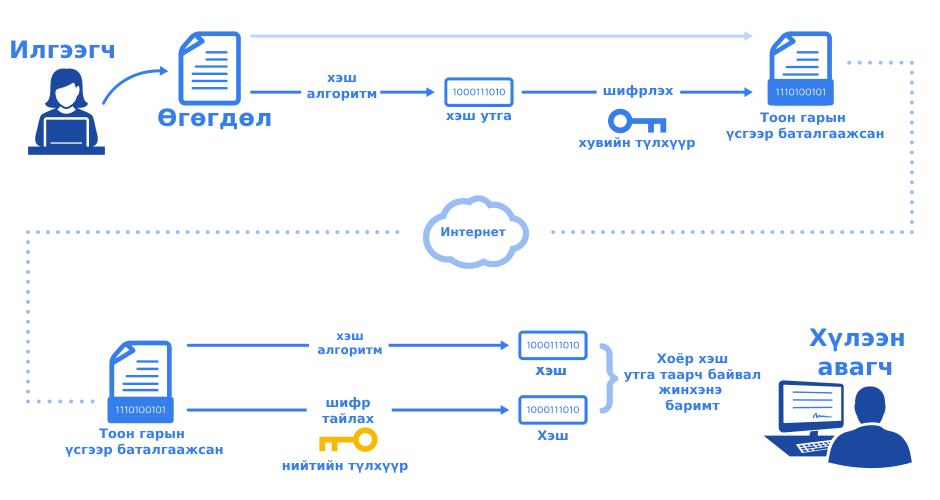
\includegraphics[scale=0.38]{src/images/dig-sign.png}
	\caption{Цахим гарын үсгийн ажиллах зарчим}
\end{figure}

\newpage
Тоон гарын үсэгт хаш функц болон хос түлхүүрийг нийлүүлж ашигласнаар, өгөгдөл илгээгчийг болон агуулгын засагдаагүй гэдгийг баталгаажуулах ажлыг зэрэг гүйцэтгэдэг юм. Блокчэйнд өмнөх хэсгийн хаш функц болон дээр өгүүлсэн цахим гарын үсгийг аль алийг нь ашигладаг бөгөөд гүйлгээ тус бүрийн үнэн зөв байдал, нийцтэй байдлын талаарх мэдээллийн илгээгч, агуулгын бүрэн бүтэн(засагдаагүй) байдлын баталгаа зэрэг төрөл бүрийн зорилгоор ашигладаг.

\subsection{Ухаалаг гэрээ}
Ухаалаг гэрээ гэдэг нь дундын зуучлагч буюу хуульч, нотариатгүйгээр хоёр этгээд гэрээ байгуулсныг баталсан компьютерын код бөгөөд тухайн гэрээний нөхцөл, үүрэг, хариуцлагыг багтаасан байна. Анх этереум нь ухаалаг гэрээг оруулсан блокчэйн гэдгийг гаргаж, түүний дараагаар олон тооны блокчэйнд ухаалаг гэрээг оруулж ирсэн. Ухаалаг гэрээ нь зөвхөн нөхцөл, үүргийг заахаас гадна автоматаар биелэх боломжтой байдаг.

Анх 1996 онд Nick Szabo  ухаалаг гэрээний санааг нь гаргаж ирсэн. Гол санаа нь хүнээс хамааралгүйгээр урьдчилан тодорхойлсон ямар нэг нөхцөлийн биелэх үед автоматаар үйлдэл хийгдэнэ.

\begin{enumerate}
   \item  Хийгдсэн үйлдэл/гүйлгээ нь олон нийтэд ил байх ч, хэн хийсэн бэ гэдэг нь нууц байж болдог.
   \item  Блокчэйн сүлжээний бүх зангилаанууд ухаалаг гэрээг ажиллуулдаг.
   \item Цаг хугацаа хэмнэхээс гадна гарч болох олон асуудлыг шийдэх боломжтой. (3-дагч этгээдийг оролцоо хэрэггүй)
\end{enumerate}

\subsection{Блокчэйн зарим хэрэглээ}
Олон улсын хэмжээнд стартап компаниуд блокчэйн технологийг ашигласан шинэ системийг эрүүл мэнд, даатгал, татвар зэрэг олон салбарт санал болгож байна.

Жишээлбэл, \textbf{Нэгдсэн Үндэстний Байгууллага} 2017 онд блокчэйн технологи
ашигласан олон төрлийн санал, санаачилагыг хэрэгжүүлснээс үүний нэг болох тусламж түгээлтийн бүртгэлийн систем амжилттай хэрэгжсэн байна. НҮБ-аас гаргасан судалгаагаар, нийт тусламжийн 30 орчим хувь нь очих ёстой хүлээн авагчдаа хүрдэггүй гэж гарсан байна. 2017 оны тавдугаар сараас НҮБ-ын Дэлхийн хүнсний хөтөлбөрт хэрэгжсэн хүрээнд Сирийн дүрвэгчдэд үзүүлж байгаа тусламжийг этереум блокчэйн ашиглаж түгээжээ. Тодруулбал, Иордан улсын дүрвэгчдийн хуаранд байрлаж байгаа Сири улсын 10500 дүрвэгчид хүнсний бүтээгдэхүүн (1.4 сая ам.доллар) түгээхэд криптовалютад суурилсан ваучер тарааж, уг ваучераа ашиглан хуаранд байрлах дэлгүүрээс хүнсний бүтээгдэхүүн авах боломжийг хангажээ. НҮБ-аас уг төслийг өмнөх тусламжтай харьцуулахад маш амжилттай хэрэгжсэн гэж үзэж байгаа бөгөөд 2018 оны хоёрдугаар улиралд тусламжинд хамрагдах хүний тоог 500,000-д хүргэхээр төлөвлөж байна гэж мэдээлж байна.

НҮБ-аас хамгийн сүүлд эхлүүлсэн нэг ажил нь хүүхдийг блокчэйнд бүртгэлжүүлэх систем юм. Хуурамч бичиг баримт үйлдэн хүүхэд хил дамнуулахыг зогсооход хамгийн ээдрээтэй зүйл нь жинхэнэ юм шиг бүрдүүлсэн хуурамч бичиг баримтыг таних ажил байдаг. Хүний наймаа ихээр явагддаг бүс нутагт хүүхдүүдийг шат дараатайгаар албан ёсны бүртгэлтэй болгож, түүнийг нь НҮБ-ын блокчэйн системд хадгална. Энэ төрлийн гэмт хэрэг хамгийн их явагддаг Молдав улсад хэрэгжүүлж эхэлсэн ажээ. НҮБ-ийн судалгаагаар 5-аас доош насны хүүхэд бүртгэлжээгүй байх тохиолдол зарим бүс нутагт их байдаг байна \cite{un_child}.

\textbf{Швейцарийн Зуг (ZUG)} хот нь крипто хот болохоор ажиллаж
байгаа бөгөөд ийм уриа гаргасан бусад хот болох Сан-Франциско, Лондон, Токио, Сингапур, Нью-Иорк, Амстердамаас ялгагдах зүйл нь санхүү болон технологийн гарааны бизнесээ эхэлж буй компаниудад хууль эрх зүйн орчин нь маш тааламжтай юм. Зуг хотын удирдлага крипто хөндий байгуулж, иргэдээ блокчэйнд бүртгэж эхэлсэн ба 2017 оны арваннэгдүгээр сараас иргэддээ зориулж цахим ID авах вебийн үйлчилгээг нээсэн \cite{zug_digtal_id} нь этереум блокчэйнд суурилсан ба хэрэглэгч хаанаас ч өөрийн мэдээллийг оруулан цахим ID-гаа авах боломжтой бөгөөд хотын зүгээс уг мэдээллийг зөвхөн шалгаж баталгаажуулах эрхтэй. Энэхүү цахим ID-гаа ашиглаад иргэд зөвхөн хотын үйлчилгээг (хэрэглээний төлбөр, түрээсийн төлбөр) авахаар хязгаарлагдахгүй ба 2018 оны хавар сонгуулийн санал өгөхөд (e-vote) ашиглахаар бэлдэж байна.

\section{Дижитал эрхийн менежмент (DRM)}
Digital Rights Management (DRM) системийг дижитал контентыг хэрэглэх, тараах, хуваалцахад хяналт тавих зорилготой технологиуд гэж ойлгож болно. Энэ нь ном, хөгжим, кино, программ хангамж зэрэг дижитал контентыг хамгаалах, агуулгын эзэмшигч, хэвлэн нийтлэгчдийн оюуны өмчийн эрхийг хамгаалахад чиглэдэг \cite{drm}.

\subsection{DRM-ийн үндсэн ойлголт ба бүрэлдэхүүн хэсгүүд:}
\begin{itemize}
   \item \textbf{Шифрлэлт:} Шифрлэлт нь криптограф алгоритмыг ашиглан цахим контентыг унших боломжгүй формат руу хөрвүүлэх явдал юм. Шифрлэгдсэн контентод зөвхөн шаардлагатай код тайлах түлхүүрийг эзэмшсэн эрх бүхий хэрэглэгчид хандах буюу тайлж болно.

    \item \textbf{Хандалтын хяналт:} DRM систем нь дижитал контент руу хэн хандах, үзэх, өөрчлөх, түгээх боломжтойг зохицуулах хандалтын хяналтын механизмыг хэрэгжүүлдэг. Хандалтын эрхийг ихэвчлэн хэрэглэгчийн үүрэг, лиценз эсвэл контент эзэмшигчээс олгосон зөвшөөрөл дээр үндэслэн тодорхойлдог.

    \item \textbf{Лицензийн менежмент:} DRM шийдлүүд нь хэрэглэгчдэд дижитал контент руу нэвтрэх, ашиглах зөвшөөрөл олгохын тулд лицензэд суурилсан загваруудыг ашигладаг. Лицензүүд нь ашиглалтын хугацаа, зөвшөөрөгдсөн төхөөрөмж, нэгэн зэрэг хэрэглэгчдийн тоо зэрэг ашиглалтын нөхцөл, нөхцөлийг тодорхойлдог.

    \item \textbf{Тоон усан тэмдэг:} Тоон усан тэмдэг нь үл үзэгдэх танигч эсвэл гарын үсгийг цахим контентод  оруулахад ашигладаг техник юм. Усан тэмдэглэгээг контентын зөвшөөрөлгүй хуулбарыг эх сурвалж руу нь буцаах эсвэл контентын жинхэнэ эсэхийг шалгахад ашиглаж болно.

    \item \textbf{Хуулбарлах хамгаалалт:} DRM системүүд нь цахим контентыг зөвшөөрөлгүй хуулбарлах, хуулбарлахаас сэргийлэхийн тулд хуулбарлах хамгаалалтын механизмыг хэрэгжүүлдэг. Хулгайлах, зөвшөөрөлгүй түгээхээс урьдчилан сэргийлэхийн тулд хуулбарлахаас урьдчилан сэргийлэх, хуулбарлах хяналт, хуулбар илрүүлэх зэрэг арга техникийг ашигладаг.
\end{itemize}

\section{DRM систем дэх блокчэйн технологийн боломжууд}
Блокчейн технологи нь төвлөрсөн бус, ил тод, өөрчлөх боломжгүй шинж чанартай бөгөөд уламжлалт дижитал эрхийн менежментийн (DRM) системийн тулгардаг олон асуудлыг шийдвэрлэх боломжтой. Үүнд:
\begin{enumerate}
   \item \textbf{Төвлөрсөн бус өмчлөлийн болон гарал үүслийн бүртгэл:} Блокчейн технологи нь дижитал хөрөнгийн өмчлөл болон гарал үүслийг өөрчлөх боломжгүй, төвлөрсөн бус бүртгэлийг хангаж чадна. Ингэснээр зохиогч болон эзэмшигч нар зохих хүлээн зөвшөөрөл, нөхөн төлбөрийг авах боломжтой бөгөөд хөрөнгийн өмчлөл болон шилжүүлгийн түүхийг ил тод байдлаар хянах боломжтой болно. Энэ нь уламжлалт DRM системд тулгардаг өмчлөлийн эргэлзээ болон ил тод бус байдлын асуудлыг шийдвэрлэнэ.
   \item \textbf{Ухаалаг гэрээгээр дамжуулан эрхийн автоматжуулсан менежмент:} Блокчейн дээр суурилсан ухаалаг гэрээнүүд нь дижитал хөрөнгийн хэрэглээ, роялти төлбөр тооцоо болон бусад холбогдох нөхцөлүүдийг автоматаар хэрэгжүүлэх боломжтой. Эдгээр нь өөрөө гүйцэтгэгддэг гэрээнүүд нь зөвхөн ил тод, үнэн зөв байдлыг хангаад зогсохгүй тохиролцсон нөхцөлүүдийг автоматаар хэрэгжүүлж, оролцогч талуудын итгэлцлийг нэмэгдүүлнэ.
   \item \textbf{Хэрэглэгчийн хяналт ба эрх мэдэл:}
   Блокчейн технологид суурилсан дижитал хөрөнгийн менежментийн систем нь хэрэглэгчдэд хөрөнгийн хандах эрхийн зөвшөөрөл, өмчлөх эрхийг шилжүүлэх, дахин зарах зэрэг хяналтыг олгож, шинэ бизнес загваруудыг хэрэгжүүлэх боломжийг олгоно. Энэ нь хэрэглэгчийн эрх мэдэл, хяналтын дутагдлыг шийдвэрлэж, уламжлалт DRM системд тулгардаг асуудлыг арилгана.
   \item \textbf{Төлбөр тооцоо ба мөнгө олох шинэ загварууд:}
   Блокчейн нь  төлбөр тооцоог хөнгөвчлөх чадвар нь ашиглалтын төлбөр эсвэл захиалгад суурилсан хандалт зэрэг дижитал контентоор мөнгө олох шинэ загваруудыг бий болгож чадна. Энэ нь уламжлалт DRM загвартай харьцуулахад илүү уян хатан, хэрэглэгчдэд ээлтэй сонголтуудыг өгөх боломжтой.
\end{enumerate}

\section{Технологийн судалгаа}
\subsection{React \& Next.js}
\subsubsection{Declarative}
React нь хэрэглэгчийн интерактив интерфейс бүтээхийг хялбарчилдаг. Aппликейшны state бүрд зориулсан энгийн бүтэц зохион байгуулахаас гадна, React нь өгөгдөл өөрчлөгдөхөд яг зөв компонентоо өөрчлөн рендер хийдэг. Declarative бүтэц нь кодыг тань debug хийхэд хялбар болгохоос гадна, ажиллагаа нь илүү тодорхой болдог.

\subsubsection{Next.js}
Netflix, TikTok, Hulu, Twitch, Nike гэсэн орчин үеийн аваргууд ашигладаг энэхүү орчин үеийн фрэймворк нь React технологи дээр үндэслэгдсэн бөгөөд Frontend, Backend хоёр талд хоёуланд нь ажилладаг веб аппуудыг хийх чадвартайгаараа бусдаасаа давуу юм. Next.js-ийн үндсэн дизайн нь клиент болон сервер талын аль алиных давуу талыг ашиглаж чаддаг, ямар нэг дутагдалгүй веб сайтыг яаж хамгийн хурдан хялбар бүтээх вэ гэдгийг бодож тусгасан байдаг. Next.js нь сервер талд react компонентуудыг рендерлэн энгийн html, css, json файл болгон хувиргах замаар ажилладаг бөгөөд 2020 оноос олон нийтэд танигдсан JAMStack технологи болон статик сайт, автоматаар статик хуудас үүсгэх, CDN deployment, сервергүй функц, тэг тохиргоо, файлын системийн рүүтинг (PHP-ээс санаа авсан), SWR (stale while revalidate), сервер талд рендерлэх зэрэг асар олон орчин үеийн шинэхэн технологиудыг бүгдийг хийж чаддаг анхны бүрэн веб фрэймворк гэж хэлж болно.

\subsection{Ethereum блокчэйн}
Төвлөрсөн бус, блокчэйн дээр суурилсан программуудыг хангамжийн платформ анх Ethereum-ийг 2013 онд программист Vitalik Buterin бичсэн бөгөөд 2015 онд олон нийтэд анх танилцуулагдсан юм. Ethereum нь бусад койныг бодвол зөвхөн арилжааны бус тус платформыг ашиглан smart contract буюу ухаалаг гэрээ үүсгэх боломжтой. Энэ нь энгийнээр хөгжүүлэгчдэд төвлөрсөн бус хэрэглээний программуудыг бүтээх, ажиллуулах боломжийг олгодог.

\subsection{Hardhat}
Hardhat нь ухаалаг гэрээг хөгжүүлэх орчин юм. Энэ нь Ethereum ухаалаг гэрээг бичих, туршихаас эхлээд байршуулах, дибаг хийх хүртэлх бүх амьдралын мөчлөгийг хөнгөвчлөх зорилготой юм. Hardhat нь Ethereum Virtual Machine (EVM) дээр бүтээгдсэн бөгөөд Ethereum, Polygon, Avalanche болон бусад EVM-тэй нийцтэй блокчэйнүүдийг дэмждэг.

\subsection{Wagmi}
Wagmi нь блокчэйнтэй ажиллахад шаардлагатай бүх зүйлийг агуулсан React Hook-ийн цуглуулга юм. Wagmi нь крифто түрийвч холбох, мэдээллийг авах, ухаалаг гэрээтэй харилцах гэх мэт үйлдлүүдийг хөнгөвчлөх боломжийг олгодог.

\subsection{IPFS \& Pinata}
IPFS буюу Interplanetary File System нь peer-to-peer сүлжээн дэх файлуудыг хадгалах, хуваалцахад зориулагдсан төвлөрсөн бус протокол юм. Үндсэндээ IPFS нь файлуудыг жижиг хэсгүүдэд хувааж, сүлжээний олон зангилаанд хадгалдаг. Энэ нь файлуудыг нэг байршилд хадгалдаггүй, харин сүлжээгээр тарааж байршуулдаг.
Pinata нь төвлөрсөн бус бичиг баримт хадгалалтын сүлжээ болох Interplanetary File System (IPFS) дээр бүтээгдсэн үйлчилгээ юм. Pinata нь хөгжүүлэгчид болон хэрэглэгчдэд IPFS сүлжээнд өгөгдөл хадгалах, уншихад хялбар болгодог. Энэ нь IPFS дээр хадгалагдсан файлуудыг байршуулах, удирдах, хандахад зориулсан API болон бусад хэрэгслээр хангаснаар IPFS-тэй харилцах үйл явцыг хялбаршуулдаг.

\subsection{Lit Protocol}
Lit Protocol нь хэрэглэгчдэд өгөгдөл шифрлэх, түүнд хандах хандалтыг хянах боломжийг олгодог төвлөрсөн бус түлхүүр удирдлагын систем юм. Lit Protocol-ийн хандалтын хяналтын систем нь хэрэглэгчид өөрсдийн өгөгдөлд хэн хандаж, ашиглах боломжтойг нарийн хянах боломжийг олгодог.
Lit Protocol-г дараах зорилгоор ашиглаж болно.
\begin{itemize}
   \item Lit сүлжээнд өгөгдлийг шифрлэх түлхүүр үүсгэх, удирдах
   \item Lit сүлжээнээс өгөгдлийн шифрлэлтийг тайлах түлхүүрийг авах эрхийг нарийвчилсан нөхцөлтэйгөөр тодорхойлох
   \item Lit сүлжээнээс түлхүүрийг авч өгөгдлийн шифрлэлтийг тайлах
\end{itemize}

Lit Protocol бол төвлөрсөн бус сүлжээ бөгөөд үйл ажиллагааны хувьд програмчлагдах түлхүүр хэлбэрээр ажилладаг. "threshold криптографи" гэж нэрлэгддэг процессоор Lit нь хувийн түлхүүрийг төвлөрсөн бус болгож, уг түлхүүр нь Lit зангилаанууд дээр тархсан байдлаар хадгалдаг.
Lit сүлжээ нь өгөгдөл шифрлэхэд BLS тоон гарын үсэг ашиглан тодорхой нөхцөл хангасан хүмүүст л шифрлэлтийг тайлахыг зөвшөөрдөг таних тэмдэгт (ID) суурилсан шифрлэлтийн схемийг ашигладаг.
BLS (Boneh-Lynn-Shacham) тоон гарын үсэг нь нийтийн түлхүүрт суурилсан криптографийн нэг төрөл бөгөөд өгөгдлийг нууцлах, баталгаажуулахад өргөн ашиглагддаг. Энэ нь тодорхой нөхцөл хангасан хүмүүст л нууцлалыг тайлах эрх олгодог тул зөвхөн зөвшөөрөгдсөн хүмүүс л өгөгдлийг үзэх боломжтой болдог.

Өгөгдөл шифрлэхийн тулд дараах алхмуудыг хийх хэрэгтэй.
\begin{enumerate}
   \item Крипто хэтэвчний гарын үсгийг авах, өөрөөр хэлбэл хэтэвчийг эзэмшдэг эсэхийг нотлох
   \item Хэн таны өгөгдлийн шифрлэлтийг тайлах түлхүүрийг авч чадах талаар хандалтын хяналтын нөхцөлийг тодорхойлох
   \item Lit сүлжээнд холбогдож, өгөгдлийг шифрлүүлэх түлхүүр үүсгэн өгөгдлийг шифрлэх
\end{enumerate}

\section{Ижил төстэй системийн судалгаа}
% Audius нь дундын зуучлагчийн оролцоогүйгээр уран бүтээлчдэд хөгжмөө байршуулах, түгээх, мөнгө олох боломжийг олгодог төвлөрсөн бус платформ юм. Энэхүү платформ нь өмчлөлийг удирдах, гүйлгээг хөнгөвчлөхөд Ethereum блокчэйнийг ашигладаг бол  хөгжмийн файлуудыг төвлөрсөн бус байдлаар IPFS дээр байршуулдаг.

% OpenSea бол Ethereum блокчэйн дээр суурилсан NFT зах зээл юм. NFT буюу Non-Fungible Token нь блокчэйн технологийг ашиглан уран бүтээл, дижитал контентыг онцгой эзэмших эрхийг илэрхийлдэг токен юм. OpenSea платформоор дамжуулан хэрэглэгчид өөрсдийн NFT цуглуулгыг худалдах, худалдан авах, солилцох боломжтой.

Блокчэйн технологийг ашиглан цахим лицензийн баталгаажуулалт хийж буй хэд хэдэн системүүдийг судаллаа. Эдгээр системүүдийн ихэнх нь төвлөрсөн бус архитектур дээр суурилж, цахим бүтээгдэхүүний лицензийг баталгаажуулах, хянахад чиглэгдсэн байна.
\begin{table}[h!]
	\centering
   \begin{tabularx}{\textwidth}{|X|X|X|X|}
		\hline
      \textbf{Үзүүлэлтүүд} & \textbf{Audius} & \textbf{OpenSea} & \textbf{Манай систем}
      \\ \hline Технологи & Ethereum, Solana &	Ethereum &	Ethereum, IPFS
      \\ \hline Ухаалаг гэрээ & 	Тийм & 	Тийм & 	Тийм
      \\ \hline Хандалтын хяналт &	Тийм &	Тийм & Тийм (Lit protocol)
      \\ \hline Төвлөрсөн бус хадгалалт &	Тийм & Үгүй & Тийм (IPFS)
      \\ \hline Лицензийн төрөл & Үнэгүй болон төлбөртэй & Төлбөртэй &	Үнэгүй болон төлбөртэй
      \\ \hline Ашиглалтын төвөгтэй байдал &	Хялбар &	Хялбар &	Хялбар
      \\ \hline Хэрэгжүүлэлтийн зардал &	Дунд & Дунд & Дунд
      \\ \hline
	\end{tabularx}
   \caption{Системүүдийн харьцуулалт}
\end{table}

\subsection{Системүүдийн тайлбар}
\textbf{Audius}: Audius нь хөгжим дамжуулах үйлчилгээ бөгөөд Ethereum болон Solana блокчэйнүүдэд суурилсан. Энэ систем нь төвлөрсөн бус байдлыг хангаж, ухаалаг гэрээг ашиглан хөгжмийн бүтээлийг баталгаажуулдаг. Хэрэглэгчид үнэгүй болон төлбөртэй контентуудыг ашиглах боломжтой.

\textbf{OpenSea}: OpenSea нь дижитал бүтээл, NFT (Non-Fungible Token) худалдааны хамгийн том зах зээл бөгөөд Ethereum блокчэйнд суурилсан. Энэ систем нь ухаалаг гэрээг ашиглан дижитал өмчийг худалдах, худалдан авах боломжийг олгодог боловч төвлөрсөн хадгалалттай.

\pagebreak
\subsection{Манай системийн давуу тал}
Манай систем нь Ethereum блокчэйн дээр суурилсан бөгөөд IPFS-ийг ашиглан төвлөрсөн бус хадгалалт хийх боломжтой. Ухаалаг гэрээгээр дамжуулан лицензийн нөхцөл, хандалтын эрхийг тодорхойлох боломжтой. Мөн Lit протоколыг ашиглан хандалтын хяналтын нөхцөлийг хэрэгжүүлэх боломжтой. Энэ нь хэрэглэгчид болон бүтээлийн эзэд хоорондын итгэлцлийг нэмэгдүүлж, цахим бүтээгдэхүүний лицензийг илүү найдвартай, аюулгүй байлгадаг.